\documentclass[twoside]{book}

% Packages required by doxygen
\usepackage{fixltx2e}
\usepackage{calc}
\usepackage{doxygen}
\usepackage[export]{adjustbox} % also loads graphicx
\usepackage{graphicx}
\usepackage[utf8]{inputenc}
\usepackage{makeidx}
\usepackage{multicol}
\usepackage{multirow}
\PassOptionsToPackage{warn}{textcomp}
\usepackage{textcomp}
\usepackage[nointegrals]{wasysym}
\usepackage[table]{xcolor}

% Font selection
\usepackage[T1]{fontenc}
\usepackage[scaled=.90]{helvet}
\usepackage{courier}
\usepackage{amssymb}
\usepackage{sectsty}
\renewcommand{\familydefault}{\sfdefault}
\allsectionsfont{%
  \fontseries{bc}\selectfont%
  \color{darkgray}%
}
\renewcommand{\DoxyLabelFont}{%
  \fontseries{bc}\selectfont%
  \color{darkgray}%
}
\newcommand{\+}{\discretionary{\mbox{\scriptsize$\hookleftarrow$}}{}{}}

% Page & text layout
\usepackage{geometry}
\geometry{%
  a4paper,%
  top=2.5cm,%
  bottom=2.5cm,%
  left=2.5cm,%
  right=2.5cm%
}
\tolerance=750
\hfuzz=15pt
\hbadness=750
\setlength{\emergencystretch}{15pt}
\setlength{\parindent}{0cm}
\setlength{\parskip}{3ex plus 2ex minus 2ex}
\makeatletter
\renewcommand{\paragraph}{%
  \@startsection{paragraph}{4}{0ex}{-1.0ex}{1.0ex}{%
    \normalfont\normalsize\bfseries\SS@parafont%
  }%
}
\renewcommand{\subparagraph}{%
  \@startsection{subparagraph}{5}{0ex}{-1.0ex}{1.0ex}{%
    \normalfont\normalsize\bfseries\SS@subparafont%
  }%
}
\makeatother

% Headers & footers
\usepackage{fancyhdr}
\pagestyle{fancyplain}
\fancyhead[LE]{\fancyplain{}{\bfseries\thepage}}
\fancyhead[CE]{\fancyplain{}{}}
\fancyhead[RE]{\fancyplain{}{\bfseries\leftmark}}
\fancyhead[LO]{\fancyplain{}{\bfseries\rightmark}}
\fancyhead[CO]{\fancyplain{}{}}
\fancyhead[RO]{\fancyplain{}{\bfseries\thepage}}
\fancyfoot[LE]{\fancyplain{}{}}
\fancyfoot[CE]{\fancyplain{}{}}
\fancyfoot[RE]{\fancyplain{}{\bfseries\scriptsize Generated by Doxygen }}
\fancyfoot[LO]{\fancyplain{}{\bfseries\scriptsize Generated by Doxygen }}
\fancyfoot[CO]{\fancyplain{}{}}
\fancyfoot[RO]{\fancyplain{}{}}
\renewcommand{\footrulewidth}{0.4pt}
\renewcommand{\chaptermark}[1]{%
  \markboth{#1}{}%
}
\renewcommand{\sectionmark}[1]{%
  \markright{\thesection\ #1}%
}

% Indices & bibliography
\usepackage{natbib}
\usepackage[titles]{tocloft}
\setcounter{tocdepth}{3}
\setcounter{secnumdepth}{5}
\makeindex

% Hyperlinks (required, but should be loaded last)
\usepackage{ifpdf}
\ifpdf
  \usepackage[pdftex,pagebackref=true]{hyperref}
\else
  \usepackage[ps2pdf,pagebackref=true]{hyperref}
\fi
\hypersetup{%
  colorlinks=true,%
  linkcolor=blue,%
  citecolor=blue,%
  unicode%
}

% Custom commands
\newcommand{\clearemptydoublepage}{%
  \newpage{\pagestyle{empty}\cleardoublepage}%
}

\usepackage{caption}
\captionsetup{labelsep=space,justification=centering,font={bf},singlelinecheck=off,skip=4pt,position=top}

%===== C O N T E N T S =====

\begin{document}

% Titlepage & ToC
\hypersetup{pageanchor=false,
             bookmarksnumbered=true,
             pdfencoding=unicode
            }
\pagenumbering{roman}
\begin{titlepage}
\vspace*{7cm}
\begin{center}%
{\Large spotless\+\_\+mini\+\_\+explorer \\[1ex]\large 0.\+1 }\\
\vspace*{1cm}
{\large Generated by Doxygen 1.8.11}\\
\end{center}
\end{titlepage}
\clearemptydoublepage
\tableofcontents
\clearemptydoublepage
\pagenumbering{arabic}
\hypersetup{pageanchor=true}

%--- Begin generated contents ---
\chapter{Hierarchical Index}
\section{Class Hierarchy}
This inheritance list is sorted roughly, but not completely, alphabetically\+:\begin{DoxyCompactList}
\item \contentsline{section}{frontier\+Ops}{\pageref{classfrontierOps}}{}
\begin{DoxyCompactList}
\item \contentsline{section}{path\+Planner}{\pageref{classpathPlanner}}{}
\end{DoxyCompactList}
\end{DoxyCompactList}

\chapter{Class Index}
\section{Class List}
Here are the classes, structs, unions and interfaces with brief descriptions\+:\begin{DoxyCompactList}
\item\contentsline{section}{\hyperlink{classfrontierOps}{frontier\+Ops} \\*The \hyperlink{classfrontierOps}{frontier\+Ops} class. It forms the base class and \hyperlink{classpathPlanner}{path\+Planner} class inherits from it. It mainly has methods to process Frontiers in a map }{\pageref{classfrontierOps}}{}
\item\contentsline{section}{\hyperlink{classpathPlanner}{path\+Planner} \\*Path planner class }{\pageref{classpathPlanner}}{}
\end{DoxyCompactList}

\chapter{File Index}
\section{File List}
Here is a list of all documented files with brief descriptions\+:\begin{DoxyCompactList}
\item\contentsline{section}{include/spotless\+\_\+mini\+\_\+explorer/\hyperlink{frontierOps_8hpp}{frontier\+Ops.\+hpp} \\*Here all the class variables and methods are declared. \hyperlink{classfrontierOps}{frontier\+Ops} is the base class for the system and provides helper functions to process the map obtained of the surrounding. Broadly speaking it receives the map and sends back the point cloud of medians of the frontiers so that the base class can now use that information to set a goal for the bot and move it there }{\pageref{frontierOps_8hpp}}{}
\item\contentsline{section}{include/spotless\+\_\+mini\+\_\+explorer/\hyperlink{pathPlanner_8hpp}{path\+Planner.\+hpp} \\*Here all the class variables and methods are declared. \hyperlink{classpathPlanner}{path\+Planner} is the derived class (inherits from the \hyperlink{classfrontierOps}{frontier\+Ops} class). Primarily, this class is at the front end of the system. It subscribes to the map of the surrounding and sends it to methods of the \hyperlink{classfrontierOps}{frontier\+Ops} class to process it and send the computed goal. Now it takes control again and calls the method to move the bot to the desired location }{\pageref{pathPlanner_8hpp}}{}
\item\contentsline{section}{src/\hyperlink{frontierOps_8cpp}{frontier\+Ops.\+cpp} \\*Here all the class variables and methods are defined. \hyperlink{classfrontierOps}{frontier\+Ops} is the base class for the system and provides helper functions to process the map obtained of the surrounding. Broadly speaking it receives the map and sends back the point cloud of medians of the frontiers so that the base class can now use that information to set a goal for the bot and move it there }{\pageref{frontierOps_8cpp}}{}
\item\contentsline{section}{src/\hyperlink{pathPlanner_8cpp}{path\+Planner.\+cpp} \\*Here all the class variables and methods are defined. \hyperlink{classpathPlanner}{path\+Planner} is the derived class (inherits from the \hyperlink{classfrontierOps}{frontier\+Ops} class). Primarily, this class is at the front end of the system. It subscribes to the map of the surrounding and sends it to methods of the \hyperlink{classfrontierOps}{frontier\+Ops} class to process it and send the computed goal. Now it takes control again and calls the method to move the bot to the desired location }{\pageref{pathPlanner_8cpp}}{}
\item\contentsline{section}{test/\hyperlink{testFrontierOps_8cpp}{test\+Frontier\+Ops.\+cpp} \\*Frontier Ops is the base class and has important functions related to processing the frontiers. In this file we wish to test the functions of this class which can be isolated. Futher developments will be made }{\pageref{testFrontierOps_8cpp}}{}
\item\contentsline{section}{test/\hyperlink{testPathPlanner_8cpp}{test\+Path\+Planner.\+cpp} \\*Path Planner class is the derived class and primarily takes care of the call back function, for getting the map of the surrounding, and moving the robot }{\pageref{testPathPlanner_8cpp}}{}
\end{DoxyCompactList}

\chapter{Class Documentation}
\hypertarget{classfrontierOps}{}\section{frontier\+Ops Class Reference}
\label{classfrontierOps}\index{frontier\+Ops@{frontier\+Ops}}


The \hyperlink{classfrontierOps}{frontier\+Ops} class. It forms the base class and \hyperlink{classpathPlanner}{path\+Planner} class inherits from it. It mainly has methods to process Frontiers in a map.  




{\ttfamily \#include $<$frontier\+Ops.\+hpp$>$}



Inheritance diagram for frontier\+Ops\+:
\nopagebreak
\begin{figure}[H]
\begin{center}
\leavevmode
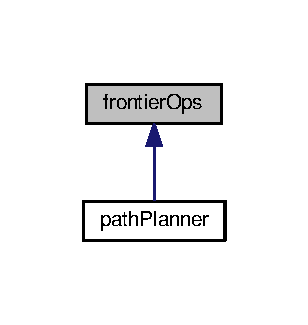
\includegraphics[width=148pt]{classfrontierOps__inherit__graph}
\end{center}
\end{figure}
\subsection*{Public Member Functions}
\begin{DoxyCompactItemize}
\item 
\hyperlink{classfrontierOps_a8c0a23673e5f301bd3ced6bed48e9a68}{frontier\+Ops} ()
\begin{DoxyCompactList}\small\item\em Constructor for class. Left empty for future development. \end{DoxyCompactList}\item 
std\+::vector$<$ std\+::vector$<$ int $>$ $>$ \hyperlink{classfrontierOps_afccdd525011a5e5612e508b1cc3f970c}{process\+Frontiers} (const nav\+\_\+msgs\+::\+Occupancy\+Grid \&map, int map\+Height, int map\+Width, int pose)
\begin{DoxyCompactList}\small\item\em Takes in the map and finds out the potential frontiers by doing a breadth first search. It uses a queue to maintain the frontiers. Makes calls to other methods of the class as a part of computing the frontiers. \end{DoxyCompactList}\item 
bool \hyperlink{classfrontierOps_a7b683fae50c4177ff4a03a8d7f81135e}{is\+Frontier} (const nav\+\_\+msgs\+::\+Occupancy\+Grid \&map, int point, int map\+Size, int map\+Width)
\begin{DoxyCompactList}\small\item\em Checks if a given point on a given map is a frontier or not. Checks the occupancy grid values of the point ad its neighbours and determines whether or not it is a frontier. \end{DoxyCompactList}\item 
void \hyperlink{classfrontierOps_a50425855de4624cdd70b521e27a77306}{get\+Adjacent\+Pts} (int $\ast$loc, int position, int map\+Width)
\begin{DoxyCompactList}\small\item\em Receives a pointer to an empty array and a point. It fills the array with eight adjacent neighbours of the point on a given map. \end{DoxyCompactList}\item 
int \hyperlink{classfrontierOps_a1d13d033b937ae062daeeec85f7cde89}{get\+Nearest\+Frontier} (const sensor\+\_\+msgs\+::\+Point\+Cloud frontier\+Cloud)
\begin{DoxyCompactList}\small\item\em Get the nearest frontier (euclidean distance) \end{DoxyCompactList}\item 
int \hyperlink{classfrontierOps_a565ae2e8f1b0b957014c740e3358b794}{get\+Farthest\+Frontier} (const sensor\+\_\+msgs\+::\+Point\+Cloud frontier\+Cloud)
\begin{DoxyCompactList}\small\item\em At times when the bot fails to move to a nearby frontier we can move it all the way to the farthest frontier to cover more area. \end{DoxyCompactList}\item 
float \hyperlink{classfrontierOps_a00b0353fd53b19d709e14a951a85637e}{get\+Distance} (float x1, float x2, float y1, float y2)
\begin{DoxyCompactList}\small\item\em Get euclidean distance between two points. \end{DoxyCompactList}\item 
\hyperlink{classfrontierOps_ade1dc1a2a60cb389520936567ab78e0d}{$\sim$frontier\+Ops} ()\hypertarget{classfrontierOps_ade1dc1a2a60cb389520936567ab78e0d}{}\label{classfrontierOps_ade1dc1a2a60cb389520936567ab78e0d}

\begin{DoxyCompactList}\small\item\em Destructor for class \hyperlink{classfrontierOps}{frontier\+Ops}. Left empty for future development. \end{DoxyCompactList}\end{DoxyCompactItemize}


\subsection{Detailed Description}
The \hyperlink{classfrontierOps}{frontier\+Ops} class. It forms the base class and \hyperlink{classpathPlanner}{path\+Planner} class inherits from it. It mainly has methods to process Frontiers in a map. 

\subsection{Constructor \& Destructor Documentation}
\index{frontier\+Ops@{frontier\+Ops}!frontier\+Ops@{frontier\+Ops}}
\index{frontier\+Ops@{frontier\+Ops}!frontier\+Ops@{frontier\+Ops}}
\subsubsection[{\texorpdfstring{frontier\+Ops()}{frontierOps()}}]{\setlength{\rightskip}{0pt plus 5cm}frontier\+Ops\+::frontier\+Ops (
\begin{DoxyParamCaption}
{}
\end{DoxyParamCaption}
)}\hypertarget{classfrontierOps_a8c0a23673e5f301bd3ced6bed48e9a68}{}\label{classfrontierOps_a8c0a23673e5f301bd3ced6bed48e9a68}


Constructor for class. Left empty for future development. 

\begin{DoxyReturn}{Returns}
None 
\end{DoxyReturn}


\subsection{Member Function Documentation}
\index{frontier\+Ops@{frontier\+Ops}!get\+Adjacent\+Pts@{get\+Adjacent\+Pts}}
\index{get\+Adjacent\+Pts@{get\+Adjacent\+Pts}!frontier\+Ops@{frontier\+Ops}}
\subsubsection[{\texorpdfstring{get\+Adjacent\+Pts(int $\ast$loc, int position, int map\+Width)}{getAdjacentPts(int *loc, int position, int mapWidth)}}]{\setlength{\rightskip}{0pt plus 5cm}void frontier\+Ops\+::get\+Adjacent\+Pts (
\begin{DoxyParamCaption}
\item[{int $\ast$}]{loc, }
\item[{int}]{position, }
\item[{int}]{map\+Width}
\end{DoxyParamCaption}
)}\hypertarget{classfrontierOps_a50425855de4624cdd70b521e27a77306}{}\label{classfrontierOps_a50425855de4624cdd70b521e27a77306}


Receives a pointer to an empty array and a point. It fills the array with eight adjacent neighbours of the point on a given map. 


\begin{DoxyParams}{Parameters}
{\em loc} & It\textquotesingle{}s the pointer to the starting position of an empty array \\
\hline
{\em position} & The point on the map for which we will find the adjacent neighbours \\
\hline
{\em map\+Width} & Width of the map\\
\hline
\end{DoxyParams}
\begin{DoxyReturn}{Returns}
None 
\end{DoxyReturn}
\index{frontier\+Ops@{frontier\+Ops}!get\+Distance@{get\+Distance}}
\index{get\+Distance@{get\+Distance}!frontier\+Ops@{frontier\+Ops}}
\subsubsection[{\texorpdfstring{get\+Distance(float x1, float x2, float y1, float y2)}{getDistance(float x1, float x2, float y1, float y2)}}]{\setlength{\rightskip}{0pt plus 5cm}float frontier\+Ops\+::get\+Distance (
\begin{DoxyParamCaption}
\item[{float}]{x1, }
\item[{float}]{x2, }
\item[{float}]{y1, }
\item[{float}]{y2}
\end{DoxyParamCaption}
)}\hypertarget{classfrontierOps_a00b0353fd53b19d709e14a951a85637e}{}\label{classfrontierOps_a00b0353fd53b19d709e14a951a85637e}


Get euclidean distance between two points. 


\begin{DoxyParams}{Parameters}
{\em x1} & x coordinate of point 1 \\
\hline
{\em x2} & x coordinate of point 2 \\
\hline
{\em y1} & y coordinate of point 1 \\
\hline
{\em y2} & y coordinate of point 2\\
\hline
\end{DoxyParams}
\begin{DoxyReturn}{Returns}
Euclidean distance between the points in float 
\end{DoxyReturn}
\index{frontier\+Ops@{frontier\+Ops}!get\+Farthest\+Frontier@{get\+Farthest\+Frontier}}
\index{get\+Farthest\+Frontier@{get\+Farthest\+Frontier}!frontier\+Ops@{frontier\+Ops}}
\subsubsection[{\texorpdfstring{get\+Farthest\+Frontier(const sensor\+\_\+msgs\+::\+Point\+Cloud frontier\+Cloud)}{getFarthestFrontier(const sensor_msgs::PointCloud frontierCloud)}}]{\setlength{\rightskip}{0pt plus 5cm}int frontier\+Ops\+::get\+Farthest\+Frontier (
\begin{DoxyParamCaption}
\item[{const sensor\+\_\+msgs\+::\+Point\+Cloud}]{frontier\+Cloud}
\end{DoxyParamCaption}
)}\hypertarget{classfrontierOps_a565ae2e8f1b0b957014c740e3358b794}{}\label{classfrontierOps_a565ae2e8f1b0b957014c740e3358b794}


At times when the bot fails to move to a nearby frontier we can move it all the way to the farthest frontier to cover more area. 


\begin{DoxyParams}{Parameters}
{\em frontier\+Cloud} & The point cloud created using frontier medians (center points)\\
\hline
\end{DoxyParams}
\begin{DoxyReturn}{Returns}
The frontier (number) of the farthest frontier from the point cloud 
\end{DoxyReturn}
\index{frontier\+Ops@{frontier\+Ops}!get\+Nearest\+Frontier@{get\+Nearest\+Frontier}}
\index{get\+Nearest\+Frontier@{get\+Nearest\+Frontier}!frontier\+Ops@{frontier\+Ops}}
\subsubsection[{\texorpdfstring{get\+Nearest\+Frontier(const sensor\+\_\+msgs\+::\+Point\+Cloud frontier\+Cloud)}{getNearestFrontier(const sensor_msgs::PointCloud frontierCloud)}}]{\setlength{\rightskip}{0pt plus 5cm}int frontier\+Ops\+::get\+Nearest\+Frontier (
\begin{DoxyParamCaption}
\item[{const sensor\+\_\+msgs\+::\+Point\+Cloud}]{frontier\+Cloud}
\end{DoxyParamCaption}
)}\hypertarget{classfrontierOps_a1d13d033b937ae062daeeec85f7cde89}{}\label{classfrontierOps_a1d13d033b937ae062daeeec85f7cde89}


Get the nearest frontier (euclidean distance) 


\begin{DoxyParams}{Parameters}
{\em frontier\+Cloud} & The point cloud created using frontier medians (centre points)\\
\hline
\end{DoxyParams}
\begin{DoxyReturn}{Returns}
The frontier (number) of the nearest frontier from the point cloud 
\end{DoxyReturn}
\index{frontier\+Ops@{frontier\+Ops}!is\+Frontier@{is\+Frontier}}
\index{is\+Frontier@{is\+Frontier}!frontier\+Ops@{frontier\+Ops}}
\subsubsection[{\texorpdfstring{is\+Frontier(const nav\+\_\+msgs\+::\+Occupancy\+Grid \&map, int point, int map\+Size, int map\+Width)}{isFrontier(const nav_msgs::OccupancyGrid &map, int point, int mapSize, int mapWidth)}}]{\setlength{\rightskip}{0pt plus 5cm}bool frontier\+Ops\+::is\+Frontier (
\begin{DoxyParamCaption}
\item[{const nav\+\_\+msgs\+::\+Occupancy\+Grid \&}]{map, }
\item[{int}]{point, }
\item[{int}]{map\+Size, }
\item[{int}]{map\+Width}
\end{DoxyParamCaption}
)}\hypertarget{classfrontierOps_a7b683fae50c4177ff4a03a8d7f81135e}{}\label{classfrontierOps_a7b683fae50c4177ff4a03a8d7f81135e}


Checks if a given point on a given map is a frontier or not. Checks the occupancy grid values of the point ad its neighbours and determines whether or not it is a frontier. 


\begin{DoxyParams}{Parameters}
{\em map} & Occupancy grid of the surrounding. Unknown points correspond to -\/1, obstacles have a value greater than 0 and empty space will have the value 0. It is processed like a one dimensional array. \\
\hline
{\em point} & The point in the array that needs to be checked as a frontier \\
\hline
{\em map\+Size} & Map size is map height $\ast$ map width \\
\hline
{\em map\+Width} & Width of the map\\
\hline
\end{DoxyParams}
\begin{DoxyReturn}{Returns}
True if the given point is a frontier, False if not 
\end{DoxyReturn}
\index{frontier\+Ops@{frontier\+Ops}!process\+Frontiers@{process\+Frontiers}}
\index{process\+Frontiers@{process\+Frontiers}!frontier\+Ops@{frontier\+Ops}}
\subsubsection[{\texorpdfstring{process\+Frontiers(const nav\+\_\+msgs\+::\+Occupancy\+Grid \&map, int map\+Height, int map\+Width, int pose)}{processFrontiers(const nav_msgs::OccupancyGrid &map, int mapHeight, int mapWidth, int pose)}}]{\setlength{\rightskip}{0pt plus 5cm}std\+::vector$<$ std\+::vector$<$ int $>$ $>$ frontier\+Ops\+::process\+Frontiers (
\begin{DoxyParamCaption}
\item[{const nav\+\_\+msgs\+::\+Occupancy\+Grid \&}]{map, }
\item[{int}]{map\+Height, }
\item[{int}]{map\+Width, }
\item[{int}]{pose}
\end{DoxyParamCaption}
)}\hypertarget{classfrontierOps_afccdd525011a5e5612e508b1cc3f970c}{}\label{classfrontierOps_afccdd525011a5e5612e508b1cc3f970c}


Takes in the map and finds out the potential frontiers by doing a breadth first search. It uses a queue to maintain the frontiers. Makes calls to other methods of the class as a part of computing the frontiers. 


\begin{DoxyParams}{Parameters}
{\em map} & Occupancy grid of the surrounding. Unknown points correspond to -\/1, obstacles have a value greater than 0 and empty space will have the value 0. It is processed like a one dimensional array. \\
\hline
{\em map\+Height} & Visually map is a two dimensional object but it is passed as a one dimensional array. So map\+Height is the height (or length) of the map. \\
\hline
{\em map\+Width} & Width of the map \\
\hline
{\em pose} & Pose of the robot\\
\hline
\end{DoxyParams}
\begin{DoxyReturn}{Returns}
Frontiers of type\+: a two dimensional integer vector 
\end{DoxyReturn}


The documentation for this class was generated from the following files\+:\begin{DoxyCompactItemize}
\item 
include/spotless\+\_\+mini\+\_\+explorer/\hyperlink{frontierOps_8hpp}{frontier\+Ops.\+hpp}\item 
src/\hyperlink{frontierOps_8cpp}{frontier\+Ops.\+cpp}\end{DoxyCompactItemize}

\hypertarget{classpathPlanner}{}\section{path\+Planner Class Reference}
\label{classpathPlanner}\index{path\+Planner@{path\+Planner}}


Path planner class.  




{\ttfamily \#include $<$path\+Planner.\+hpp$>$}



Inheritance diagram for path\+Planner\+:
\nopagebreak
\begin{figure}[H]
\begin{center}
\leavevmode
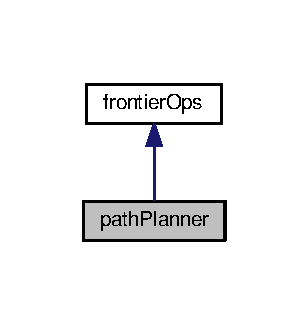
\includegraphics[width=148pt]{classpathPlanner__inherit__graph}
\end{center}
\end{figure}


Collaboration diagram for path\+Planner\+:
\nopagebreak
\begin{figure}[H]
\begin{center}
\leavevmode
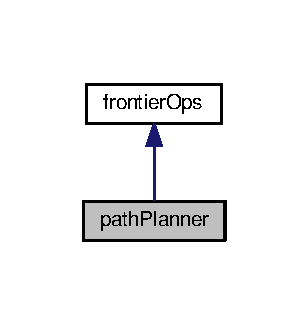
\includegraphics[width=148pt]{classpathPlanner__coll__graph}
\end{center}
\end{figure}
\subsection*{Public Member Functions}
\begin{DoxyCompactItemize}
\item 
\hyperlink{classpathPlanner_aff1bbc2236712fb764100cebe851c3ed}{path\+Planner} ()\hypertarget{classpathPlanner_aff1bbc2236712fb764100cebe851c3ed}{}\label{classpathPlanner_aff1bbc2236712fb764100cebe851c3ed}

\begin{DoxyCompactList}\small\item\em Constructor for the \hyperlink{classpathPlanner}{path\+Planner} class. It defines the publishers of the class. \end{DoxyCompactList}\item 
void \hyperlink{classpathPlanner_a13cd0ca87b3c6f8b4ade900df966e737}{map\+Callback} (const nav\+\_\+msgs\+::\+Occupancy\+Grid \&map)
\begin{DoxyCompactList}\small\item\em This is the call back function of the map subscriber. \end{DoxyCompactList}\item 
void \hyperlink{classpathPlanner_acbe410097020c8f6073a9a19ef8fc68e}{full\+Scan} ()
\begin{DoxyCompactList}\small\item\em Method to make the bot rotate 360 degrees and get a sweep scan of the surrounding. This is called in the beginning to get the initial understanding of the environment. \end{DoxyCompactList}\item 
void \hyperlink{classpathPlanner_a2455be4e0454389304f9835b5e8ccfae}{update\+Map} ()
\begin{DoxyCompactList}\small\item\em Sets the map subscriber to the correct topic. \end{DoxyCompactList}\item 
void \hyperlink{classpathPlanner_a442f9f0d8c9e38ac3e1962a005d2e18a}{move\+Bot} (const sensor\+\_\+msgs\+::\+Point\+Cloud frontier\+Cloud)
\begin{DoxyCompactList}\small\item\em This is where the magic happens. At the end of every iteration of scanning and processing, the system generates a point cloud of frontiers. This method sets the goal as the nearest frontier for the bot using the move base package. In case the execution was not successful, which should be rare, it tries to go to the farthest frontier. \end{DoxyCompactList}\item 
int \hyperlink{classpathPlanner_a2600d05e907410f3c0cf6718425c5cee}{get\+Median} (std\+::vector$<$ int $>$ frontier)
\begin{DoxyCompactList}\small\item\em Receives the array of frontier points and it sends back the centre point of the frontier. \end{DoxyCompactList}\item 
\hyperlink{classpathPlanner_adca2c6ed8e4505daf4f49f64f3319261}{$\sim$path\+Planner} ()\hypertarget{classpathPlanner_adca2c6ed8e4505daf4f49f64f3319261}{}\label{classpathPlanner_adca2c6ed8e4505daf4f49f64f3319261}

\begin{DoxyCompactList}\small\item\em Destructor for class \hyperlink{classpathPlanner}{path\+Planner}. Left empty for future development. \end{DoxyCompactList}\end{DoxyCompactItemize}


\subsection{Detailed Description}
Path planner class. 

\subsection{Member Function Documentation}
\index{path\+Planner@{path\+Planner}!full\+Scan@{full\+Scan}}
\index{full\+Scan@{full\+Scan}!path\+Planner@{path\+Planner}}
\subsubsection[{\texorpdfstring{full\+Scan()}{fullScan()}}]{\setlength{\rightskip}{0pt plus 5cm}void path\+Planner\+::full\+Scan (
\begin{DoxyParamCaption}
{}
\end{DoxyParamCaption}
)}\hypertarget{classpathPlanner_acbe410097020c8f6073a9a19ef8fc68e}{}\label{classpathPlanner_acbe410097020c8f6073a9a19ef8fc68e}


Method to make the bot rotate 360 degrees and get a sweep scan of the surrounding. This is called in the beginning to get the initial understanding of the environment. 


\begin{DoxyParams}{Parameters}
{\em None} & \\
\hline
\end{DoxyParams}
\begin{DoxyReturn}{Returns}
None 
\end{DoxyReturn}
\index{path\+Planner@{path\+Planner}!get\+Median@{get\+Median}}
\index{get\+Median@{get\+Median}!path\+Planner@{path\+Planner}}
\subsubsection[{\texorpdfstring{get\+Median(std\+::vector$<$ int $>$ frontier)}{getMedian(std::vector< int > frontier)}}]{\setlength{\rightskip}{0pt plus 5cm}int path\+Planner\+::get\+Median (
\begin{DoxyParamCaption}
\item[{std\+::vector$<$ int $>$}]{frontier}
\end{DoxyParamCaption}
)}\hypertarget{classpathPlanner_a2600d05e907410f3c0cf6718425c5cee}{}\label{classpathPlanner_a2600d05e907410f3c0cf6718425c5cee}


Receives the array of frontier points and it sends back the centre point of the frontier. 


\begin{DoxyParams}{Parameters}
{\em frontier} & Integer array of frontier points\\
\hline
\end{DoxyParams}
\begin{DoxyReturn}{Returns}
The center point from the frontier points 
\end{DoxyReturn}
\index{path\+Planner@{path\+Planner}!map\+Callback@{map\+Callback}}
\index{map\+Callback@{map\+Callback}!path\+Planner@{path\+Planner}}
\subsubsection[{\texorpdfstring{map\+Callback(const nav\+\_\+msgs\+::\+Occupancy\+Grid \&map)}{mapCallback(const nav_msgs::OccupancyGrid &map)}}]{\setlength{\rightskip}{0pt plus 5cm}void path\+Planner\+::map\+Callback (
\begin{DoxyParamCaption}
\item[{const nav\+\_\+msgs\+::\+Occupancy\+Grid \&}]{map}
\end{DoxyParamCaption}
)}\hypertarget{classpathPlanner_a13cd0ca87b3c6f8b4ade900df966e737}{}\label{classpathPlanner_a13cd0ca87b3c6f8b4ade900df966e737}


This is the call back function of the map subscriber. 


\begin{DoxyParams}{Parameters}
{\em map} & Occupancy grid of the surrounding. Unknown points correspond to -\/1, obstacles have a value greater than 0 and empty space will have the value 0. It is processed like a one dimensional array.\\
\hline
\end{DoxyParams}
\begin{DoxyReturn}{Returns}
None 
\end{DoxyReturn}
\index{path\+Planner@{path\+Planner}!move\+Bot@{move\+Bot}}
\index{move\+Bot@{move\+Bot}!path\+Planner@{path\+Planner}}
\subsubsection[{\texorpdfstring{move\+Bot(const sensor\+\_\+msgs\+::\+Point\+Cloud frontier\+Cloud)}{moveBot(const sensor_msgs::PointCloud frontierCloud)}}]{\setlength{\rightskip}{0pt plus 5cm}void path\+Planner\+::move\+Bot (
\begin{DoxyParamCaption}
\item[{const sensor\+\_\+msgs\+::\+Point\+Cloud}]{frontier\+Cloud}
\end{DoxyParamCaption}
)}\hypertarget{classpathPlanner_a442f9f0d8c9e38ac3e1962a005d2e18a}{}\label{classpathPlanner_a442f9f0d8c9e38ac3e1962a005d2e18a}


This is where the magic happens. At the end of every iteration of scanning and processing, the system generates a point cloud of frontiers. This method sets the goal as the nearest frontier for the bot using the move base package. In case the execution was not successful, which should be rare, it tries to go to the farthest frontier. 


\begin{DoxyParams}{Parameters}
{\em frontier\+Cloud} & It\textquotesingle{}s the point cloud generated with the frontier median (centre) points\\
\hline
\end{DoxyParams}
\begin{DoxyReturn}{Returns}
None 
\end{DoxyReturn}
\index{path\+Planner@{path\+Planner}!update\+Map@{update\+Map}}
\index{update\+Map@{update\+Map}!path\+Planner@{path\+Planner}}
\subsubsection[{\texorpdfstring{update\+Map()}{updateMap()}}]{\setlength{\rightskip}{0pt plus 5cm}void path\+Planner\+::update\+Map (
\begin{DoxyParamCaption}
{}
\end{DoxyParamCaption}
)}\hypertarget{classpathPlanner_a2455be4e0454389304f9835b5e8ccfae}{}\label{classpathPlanner_a2455be4e0454389304f9835b5e8ccfae}


Sets the map subscriber to the correct topic. 


\begin{DoxyParams}{Parameters}
{\em None} & \\
\hline
\end{DoxyParams}
\begin{DoxyReturn}{Returns}
None 
\end{DoxyReturn}


The documentation for this class was generated from the following files\+:\begin{DoxyCompactItemize}
\item 
include/spotless\+\_\+mini\+\_\+explorer/\hyperlink{pathPlanner_8hpp}{path\+Planner.\+hpp}\item 
src/\hyperlink{pathPlanner_8cpp}{path\+Planner.\+cpp}\end{DoxyCompactItemize}

\chapter{File Documentation}
\hypertarget{frontierOps_8hpp}{}\section{include/spotless\+\_\+mini\+\_\+explorer/frontier\+Ops.hpp File Reference}
\label{frontierOps_8hpp}\index{include/spotless\+\_\+mini\+\_\+explorer/frontier\+Ops.\+hpp@{include/spotless\+\_\+mini\+\_\+explorer/frontier\+Ops.\+hpp}}


Here all the class variables and methods are declared. \hyperlink{classfrontierOps}{frontier\+Ops} is the base class for the system and provides helper functions to process the map obtained of the surrounding. Broadly speaking it receives the map and sends back the point cloud of medians of the frontiers so that the base class can now use that information to set a goal for the bot and move it there.  


{\ttfamily \#include $<$iostream$>$}\\*
{\ttfamily \#include $<$vector$>$}\\*
{\ttfamily \#include \char`\"{}ros/ros.\+h\char`\"{}}\\*
{\ttfamily \#include \char`\"{}sensor\+\_\+msgs/\+Point\+Cloud.\+h\char`\"{}}\\*
{\ttfamily \#include \char`\"{}nav\+\_\+msgs/\+Occupancy\+Grid.\+h\char`\"{}}\\*
Include dependency graph for frontier\+Ops.\+hpp\+:
\nopagebreak
\begin{figure}[H]
\begin{center}
\leavevmode
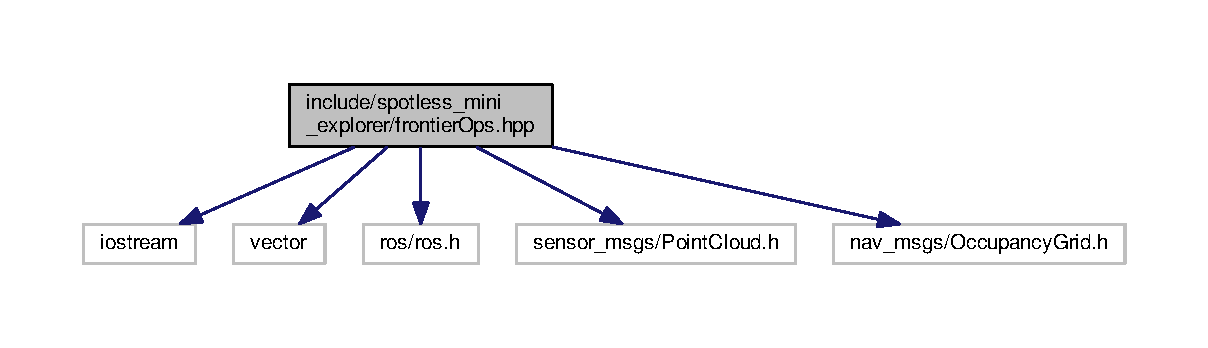
\includegraphics[width=350pt]{frontierOps_8hpp__incl}
\end{center}
\end{figure}
This graph shows which files directly or indirectly include this file\+:
\nopagebreak
\begin{figure}[H]
\begin{center}
\leavevmode
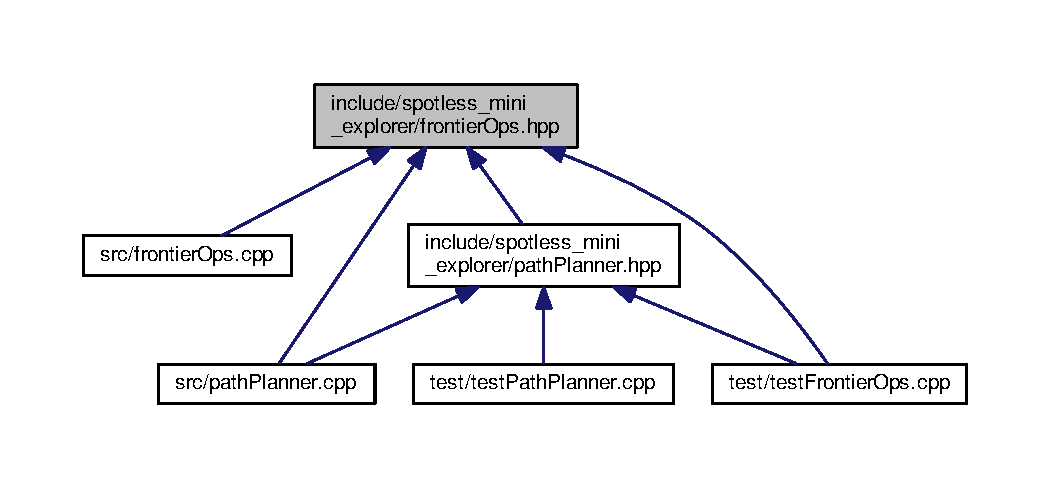
\includegraphics[width=350pt]{frontierOps_8hpp__dep__incl}
\end{center}
\end{figure}
\subsection*{Classes}
\begin{DoxyCompactItemize}
\item 
class \hyperlink{classfrontierOps}{frontier\+Ops}
\begin{DoxyCompactList}\small\item\em The \hyperlink{classfrontierOps}{frontier\+Ops} class. It forms the base class and \hyperlink{classpathPlanner}{path\+Planner} class inherits from it. It mainly has methods to process Frontiers in a map. \end{DoxyCompactList}\end{DoxyCompactItemize}


\subsection{Detailed Description}
Here all the class variables and methods are declared. \hyperlink{classfrontierOps}{frontier\+Ops} is the base class for the system and provides helper functions to process the map obtained of the surrounding. Broadly speaking it receives the map and sends back the point cloud of medians of the frontiers so that the base class can now use that information to set a goal for the bot and move it there. 

M\+IT License

Copyright (c) 2018 Sarthak Mahajan

Permission is hereby granted, free of charge, to any person obtaining a copy of this software and associated documentation files (the \char`\"{}\+Software\char`\"{}), to deal in the Software without restriction, including without limitation the rights to use, copy, modify, merge, publish, distribute, sublicense, and/or sell copies of the Software, and to permit persons to whom the Software is furnished to do so, subject to the following conditions\+:

The above copyright notice and this permission notice shall be included in all copies or substantial portions of the Software.

T\+HE S\+O\+F\+T\+W\+A\+RE IS P\+R\+O\+V\+I\+D\+ED \char`\"{}\+A\+S I\+S\char`\"{}, W\+I\+T\+H\+O\+UT W\+A\+R\+R\+A\+N\+TY OF A\+NY K\+I\+ND, E\+X\+P\+R\+E\+SS OR I\+M\+P\+L\+I\+ED, I\+N\+C\+L\+U\+D\+I\+NG B\+UT N\+OT L\+I\+M\+I\+T\+ED TO T\+HE W\+A\+R\+R\+A\+N\+T\+I\+ES OF M\+E\+R\+C\+H\+A\+N\+T\+A\+B\+I\+L\+I\+TY, F\+I\+T\+N\+E\+SS F\+OR A P\+A\+R\+T\+I\+C\+U\+L\+AR P\+U\+R\+P\+O\+SE A\+ND N\+O\+N\+I\+N\+F\+R\+I\+N\+G\+E\+M\+E\+NT. IN NO E\+V\+E\+NT S\+H\+A\+LL T\+HE A\+U\+T\+H\+O\+RS OR C\+O\+P\+Y\+R\+I\+G\+HT H\+O\+L\+D\+E\+RS BE L\+I\+A\+B\+LE F\+OR A\+NY C\+L\+A\+IM, D\+A\+M\+A\+G\+ES OR O\+T\+H\+ER L\+I\+A\+B\+I\+L\+I\+TY, W\+H\+E\+T\+H\+ER IN AN A\+C\+T\+I\+ON OF C\+O\+N\+T\+R\+A\+CT, T\+O\+RT OR O\+T\+H\+E\+R\+W\+I\+SE, A\+R\+I\+S\+I\+NG F\+R\+OM, O\+UT OF OR IN C\+O\+N\+N\+E\+C\+T\+I\+ON W\+I\+TH T\+HE S\+O\+F\+T\+W\+A\+RE OR T\+HE U\+SE OR O\+T\+H\+ER D\+E\+A\+L\+I\+N\+GS IN T\+HE S\+O\+F\+T\+W\+A\+RE. \begin{DoxyCopyright}{Copyright}
Copyright (c) 2018 Sarthak Mahajan
\end{DoxyCopyright}
\begin{DoxyAuthor}{Author}
Sarthak Mahajan 
\end{DoxyAuthor}

\hypertarget{pathPlanner_8hpp}{}\section{include/spotless\+\_\+mini\+\_\+explorer/path\+Planner.hpp File Reference}
\label{pathPlanner_8hpp}\index{include/spotless\+\_\+mini\+\_\+explorer/path\+Planner.\+hpp@{include/spotless\+\_\+mini\+\_\+explorer/path\+Planner.\+hpp}}


Here all the class variables and methods are declared. \hyperlink{classpathPlanner}{path\+Planner} is the derived class (inherits from the \hyperlink{classfrontierOps}{frontier\+Ops} class). Primarily, this class is at the front end of the system. It subscribes to the map of the surrounding and sends it to methods of the \hyperlink{classfrontierOps}{frontier\+Ops} class to process it and send the computed goal. Now it takes control again and calls the method to move the bot to the desired location.  


{\ttfamily \#include $<$iostream$>$}\\*
{\ttfamily \#include $<$vector$>$}\\*
{\ttfamily \#include \char`\"{}ros/ros.\+h\char`\"{}}\\*
{\ttfamily \#include \char`\"{}geometry\+\_\+msgs/\+Twist.\+h\char`\"{}}\\*
{\ttfamily \#include \char`\"{}nav\+\_\+msgs/\+Occupancy\+Grid.\+h\char`\"{}}\\*
{\ttfamily \#include \char`\"{}sensor\+\_\+msgs/\+Point\+Cloud.\+h\char`\"{}}\\*
{\ttfamily \#include \char`\"{}spotless\+\_\+mini\+\_\+explorer/frontier\+Ops.\+hpp\char`\"{}}\\*
Include dependency graph for path\+Planner.\+hpp\+:
\nopagebreak
\begin{figure}[H]
\begin{center}
\leavevmode
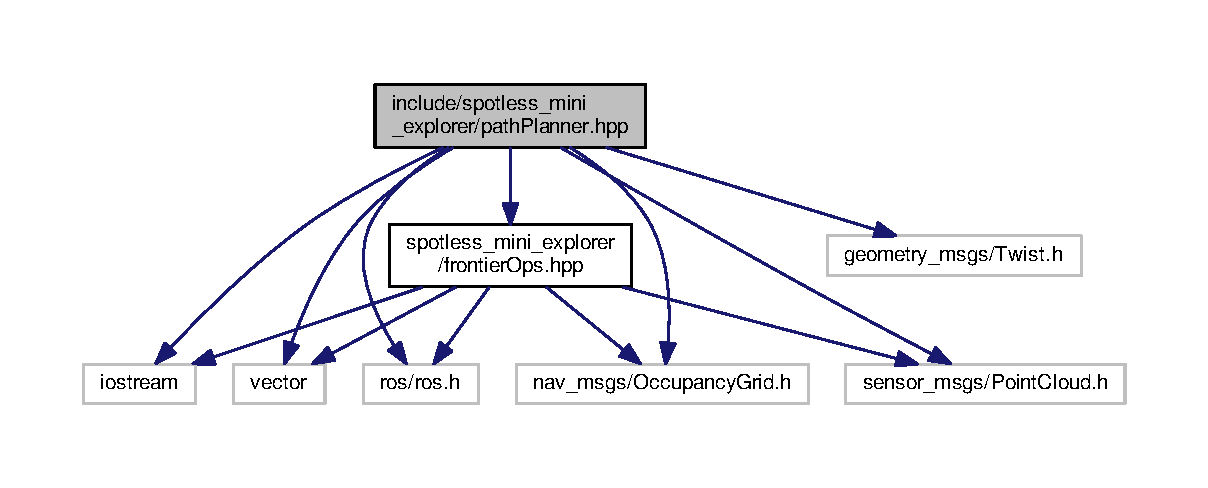
\includegraphics[width=350pt]{pathPlanner_8hpp__incl}
\end{center}
\end{figure}
This graph shows which files directly or indirectly include this file\+:
\nopagebreak
\begin{figure}[H]
\begin{center}
\leavevmode
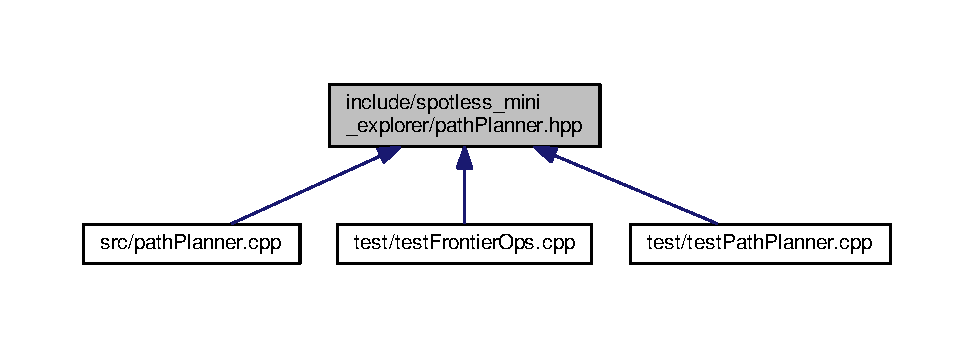
\includegraphics[width=350pt]{pathPlanner_8hpp__dep__incl}
\end{center}
\end{figure}
\subsection*{Classes}
\begin{DoxyCompactItemize}
\item 
class \hyperlink{classpathPlanner}{path\+Planner}
\begin{DoxyCompactList}\small\item\em Path planner class. \end{DoxyCompactList}\end{DoxyCompactItemize}


\subsection{Detailed Description}
Here all the class variables and methods are declared. \hyperlink{classpathPlanner}{path\+Planner} is the derived class (inherits from the \hyperlink{classfrontierOps}{frontier\+Ops} class). Primarily, this class is at the front end of the system. It subscribes to the map of the surrounding and sends it to methods of the \hyperlink{classfrontierOps}{frontier\+Ops} class to process it and send the computed goal. Now it takes control again and calls the method to move the bot to the desired location. 

M\+IT License

Copyright (c) 2018 Sarthak Mahajan

Permission is hereby granted, free of charge, to any person obtaining a copy of this software and associated documentation files (the \char`\"{}\+Software\char`\"{}), to deal in the Software without restriction, including without limitation the rights to use, copy, modify, merge, publish, distribute, sublicense, and/or sell copies of the Software, and to permit persons to whom the Software is furnished to do so, subject to the following conditions\+:

The above copyright notice and this permission notice shall be included in all copies or substantial portions of the Software.

T\+HE S\+O\+F\+T\+W\+A\+RE IS P\+R\+O\+V\+I\+D\+ED \char`\"{}\+A\+S I\+S\char`\"{}, W\+I\+T\+H\+O\+UT W\+A\+R\+R\+A\+N\+TY OF A\+NY K\+I\+ND, E\+X\+P\+R\+E\+SS OR I\+M\+P\+L\+I\+ED, I\+N\+C\+L\+U\+D\+I\+NG B\+UT N\+OT L\+I\+M\+I\+T\+ED TO T\+HE W\+A\+R\+R\+A\+N\+T\+I\+ES OF M\+E\+R\+C\+H\+A\+N\+T\+A\+B\+I\+L\+I\+TY, F\+I\+T\+N\+E\+SS F\+OR A P\+A\+R\+T\+I\+C\+U\+L\+AR P\+U\+R\+P\+O\+SE A\+ND N\+O\+N\+I\+N\+F\+R\+I\+N\+G\+E\+M\+E\+NT. IN NO E\+V\+E\+NT S\+H\+A\+LL T\+HE A\+U\+T\+H\+O\+RS OR C\+O\+P\+Y\+R\+I\+G\+HT H\+O\+L\+D\+E\+RS BE L\+I\+A\+B\+LE F\+OR A\+NY C\+L\+A\+IM, D\+A\+M\+A\+G\+ES OR O\+T\+H\+ER L\+I\+A\+B\+I\+L\+I\+TY, W\+H\+E\+T\+H\+ER IN AN A\+C\+T\+I\+ON OF C\+O\+N\+T\+R\+A\+CT, T\+O\+RT OR O\+T\+H\+E\+R\+W\+I\+SE, A\+R\+I\+S\+I\+NG F\+R\+OM, O\+UT OF OR IN C\+O\+N\+N\+E\+C\+T\+I\+ON W\+I\+TH T\+HE S\+O\+F\+T\+W\+A\+RE OR T\+HE U\+SE OR O\+T\+H\+ER D\+E\+A\+L\+I\+N\+GS IN T\+HE S\+O\+F\+T\+W\+A\+RE. \begin{DoxyCopyright}{Copyright}
Copyright (c) 2018 Sarthak Mahajan
\end{DoxyCopyright}
\begin{DoxyAuthor}{Author}
Sarthak Mahajan 
\end{DoxyAuthor}

\hypertarget{frontierOps_8cpp}{}\section{src/frontier\+Ops.cpp File Reference}
\label{frontierOps_8cpp}\index{src/frontier\+Ops.\+cpp@{src/frontier\+Ops.\+cpp}}


Here all the class variables and methods are defined. \hyperlink{classfrontierOps}{frontier\+Ops} is the base class for the system and provides helper functions to process the map obtained of the surrounding. Broadly speaking it receives the map and sends back the point cloud of medians of the frontiers so that the base class can now use that information to set a goal for the bot and move it there.  


{\ttfamily \#include $<$iostream$>$}\\*
{\ttfamily \#include $<$vector$>$}\\*
{\ttfamily \#include $<$queue$>$}\\*
{\ttfamily \#include \char`\"{}ros/ros.\+h\char`\"{}}\\*
{\ttfamily \#include \char`\"{}sensor\+\_\+msgs/\+Point\+Cloud.\+h\char`\"{}}\\*
{\ttfamily \#include \char`\"{}nav\+\_\+msgs/\+Occupancy\+Grid.\+h\char`\"{}}\\*
{\ttfamily \#include \char`\"{}tf/transform\+\_\+broadcaster.\+h\char`\"{}}\\*
{\ttfamily \#include \char`\"{}tf/transform\+\_\+listener.\+h\char`\"{}}\\*
{\ttfamily \#include \char`\"{}spotless\+\_\+mini\+\_\+explorer/frontier\+Ops.\+hpp\char`\"{}}\\*
Include dependency graph for frontier\+Ops.\+cpp\+:
\nopagebreak
\begin{figure}[H]
\begin{center}
\leavevmode
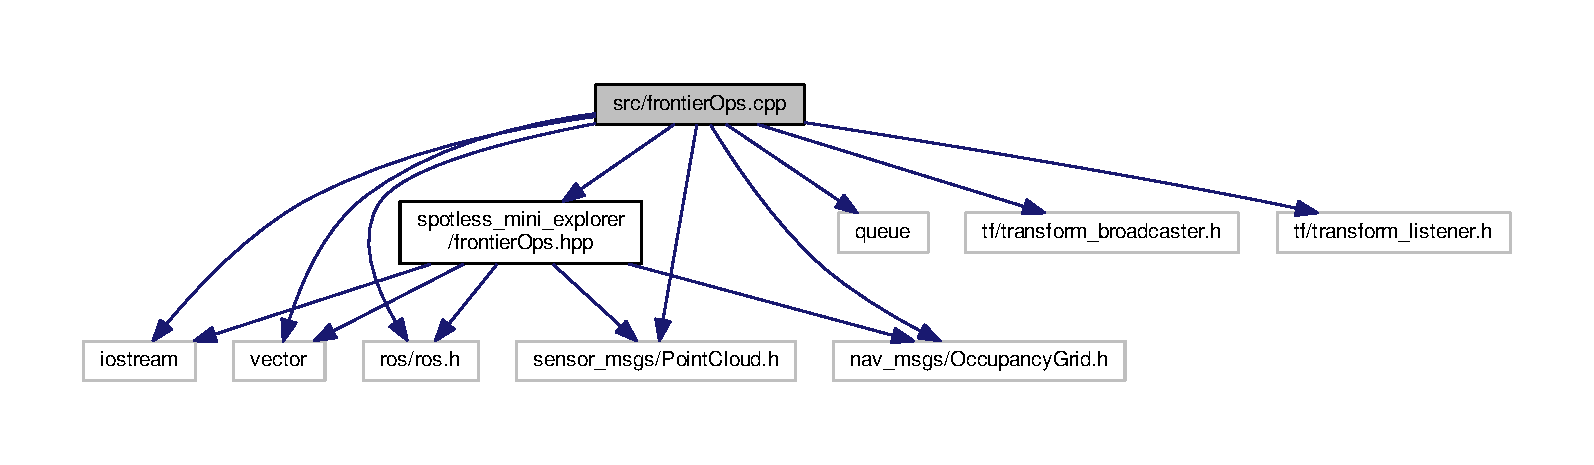
\includegraphics[width=350pt]{frontierOps_8cpp__incl}
\end{center}
\end{figure}


\subsection{Detailed Description}
Here all the class variables and methods are defined. \hyperlink{classfrontierOps}{frontier\+Ops} is the base class for the system and provides helper functions to process the map obtained of the surrounding. Broadly speaking it receives the map and sends back the point cloud of medians of the frontiers so that the base class can now use that information to set a goal for the bot and move it there. 

M\+IT License

Copyright (c) 2018 Sarthak Mahajan

Permission is hereby granted, free of charge, to any person obtaining a copy of this software and associated documentation files (the \char`\"{}\+Software\char`\"{}), to deal in the Software without restriction, including without limitation the rights to use, copy, modify, merge, publish, distribute, sublicense, and/or sell copies of the Software, and to permit persons to whom the Software is furnished to do so, subject to the following conditions\+:

The above copyright notice and this permission notice shall be included in all copies or substantial portions of the Software.

T\+HE S\+O\+F\+T\+W\+A\+RE IS P\+R\+O\+V\+I\+D\+ED \char`\"{}\+A\+S I\+S\char`\"{}, W\+I\+T\+H\+O\+UT W\+A\+R\+R\+A\+N\+TY OF A\+NY K\+I\+ND, E\+X\+P\+R\+E\+SS OR I\+M\+P\+L\+I\+ED, I\+N\+C\+L\+U\+D\+I\+NG B\+UT N\+OT L\+I\+M\+I\+T\+ED TO T\+HE W\+A\+R\+R\+A\+N\+T\+I\+ES OF M\+E\+R\+C\+H\+A\+N\+T\+A\+B\+I\+L\+I\+TY, F\+I\+T\+N\+E\+SS F\+OR A P\+A\+R\+T\+I\+C\+U\+L\+AR P\+U\+R\+P\+O\+SE A\+ND N\+O\+N\+I\+N\+F\+R\+I\+N\+G\+E\+M\+E\+NT. IN NO E\+V\+E\+NT S\+H\+A\+LL T\+HE A\+U\+T\+H\+O\+RS OR C\+O\+P\+Y\+R\+I\+G\+HT H\+O\+L\+D\+E\+RS BE L\+I\+A\+B\+LE F\+OR A\+NY C\+L\+A\+IM, D\+A\+M\+A\+G\+ES OR O\+T\+H\+ER L\+I\+A\+B\+I\+L\+I\+TY, W\+H\+E\+T\+H\+ER IN AN A\+C\+T\+I\+ON OF C\+O\+N\+T\+R\+A\+CT, T\+O\+RT OR O\+T\+H\+E\+R\+W\+I\+SE, A\+R\+I\+S\+I\+NG F\+R\+OM, O\+UT OF OR IN C\+O\+N\+N\+E\+C\+T\+I\+ON W\+I\+TH T\+HE S\+O\+F\+T\+W\+A\+RE OR T\+HE U\+SE OR O\+T\+H\+ER D\+E\+A\+L\+I\+N\+GS IN T\+HE S\+O\+F\+T\+W\+A\+RE. \begin{DoxyCopyright}{Copyright}
Copyright (c) 2018 Sarthak Mahajan
\end{DoxyCopyright}
\begin{DoxyAuthor}{Author}
Sarthak Mahajan 
\end{DoxyAuthor}

\hypertarget{pathPlanner_8cpp}{}\section{src/path\+Planner.cpp File Reference}
\label{pathPlanner_8cpp}\index{src/path\+Planner.\+cpp@{src/path\+Planner.\+cpp}}


Here all the class variables and methods are defined. \hyperlink{classpathPlanner}{path\+Planner} is the derived class (inherits from the \hyperlink{classfrontierOps}{frontier\+Ops} class). Primarily, this class is at the front end of the system. It subscribes to the map of the surrounding and sends it to methods of the \hyperlink{classfrontierOps}{frontier\+Ops} class to process it and send the computed goal. Now it takes control again and calls the method to move the bot to the desired location.  


{\ttfamily \#include $<$iostream$>$}\\*
{\ttfamily \#include $<$vector$>$}\\*
{\ttfamily \#include $<$cstdlib$>$}\\*
{\ttfamily \#include \char`\"{}ros/ros.\+h\char`\"{}}\\*
{\ttfamily \#include \char`\"{}geometry\+\_\+msgs/\+Twist.\+h\char`\"{}}\\*
{\ttfamily \#include \char`\"{}nav\+\_\+msgs/\+Occupancy\+Grid.\+h\char`\"{}}\\*
{\ttfamily \#include \char`\"{}sensor\+\_\+msgs/\+Point\+Cloud.\+h\char`\"{}}\\*
{\ttfamily \#include \char`\"{}tf/transform\+\_\+broadcaster.\+h\char`\"{}}\\*
{\ttfamily \#include \char`\"{}tf/transform\+\_\+listener.\+h\char`\"{}}\\*
{\ttfamily \#include \char`\"{}move\+\_\+base\+\_\+msgs/\+Move\+Base\+Action.\+h\char`\"{}}\\*
{\ttfamily \#include \char`\"{}actionlib/client/simple\+\_\+action\+\_\+client.\+h\char`\"{}}\\*
{\ttfamily \#include \char`\"{}spotless\+\_\+mini\+\_\+explorer/path\+Planner.\+hpp\char`\"{}}\\*
{\ttfamily \#include \char`\"{}spotless\+\_\+mini\+\_\+explorer/frontier\+Ops.\+hpp\char`\"{}}\\*
Include dependency graph for path\+Planner.\+cpp\+:
\nopagebreak
\begin{figure}[H]
\begin{center}
\leavevmode
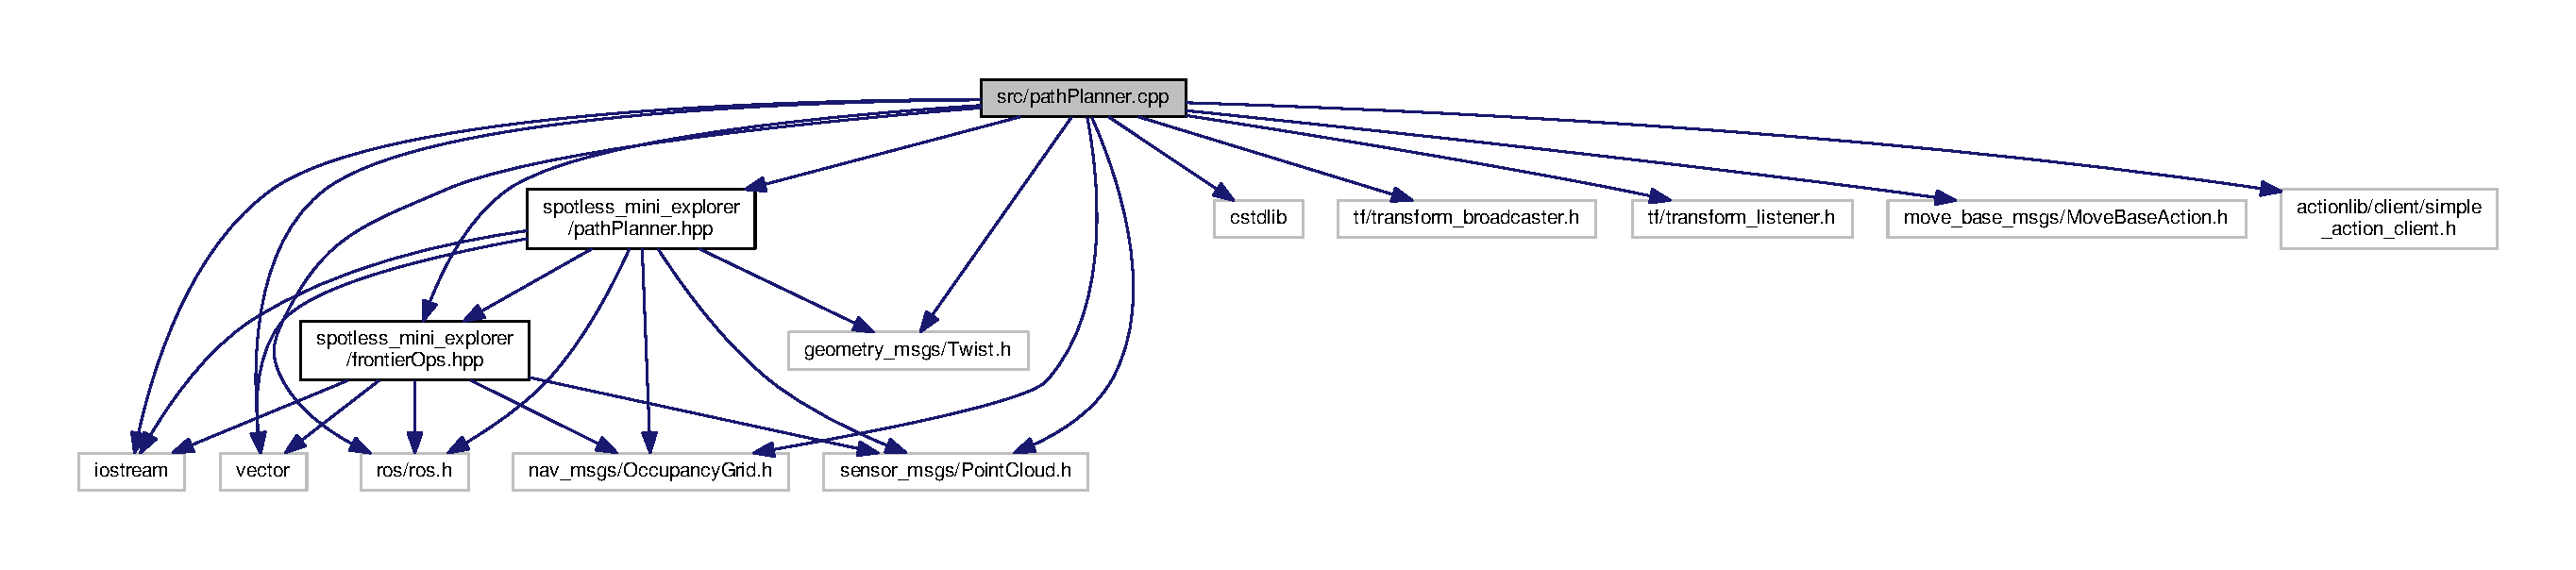
\includegraphics[width=350pt]{pathPlanner_8cpp__incl}
\end{center}
\end{figure}


\subsection{Detailed Description}
Here all the class variables and methods are defined. \hyperlink{classpathPlanner}{path\+Planner} is the derived class (inherits from the \hyperlink{classfrontierOps}{frontier\+Ops} class). Primarily, this class is at the front end of the system. It subscribes to the map of the surrounding and sends it to methods of the \hyperlink{classfrontierOps}{frontier\+Ops} class to process it and send the computed goal. Now it takes control again and calls the method to move the bot to the desired location. 

M\+IT License

Copyright (c) 2018 Sarthak Mahajan

Permission is hereby granted, free of charge, to any person obtaining a copy of this software and associated documentation files (the \char`\"{}\+Software\char`\"{}), to deal in the Software without restriction, including without limitation the rights to use, copy, modify, merge, publish, distribute, sublicense, and/or sell copies of the Software, and to permit persons to whom the Software is furnished to do so, subject to the following conditions\+:

The above copyright notice and this permission notice shall be included in all copies or substantial portions of the Software.

T\+HE S\+O\+F\+T\+W\+A\+RE IS P\+R\+O\+V\+I\+D\+ED \char`\"{}\+A\+S I\+S\char`\"{}, W\+I\+T\+H\+O\+UT W\+A\+R\+R\+A\+N\+TY OF A\+NY K\+I\+ND, E\+X\+P\+R\+E\+SS OR I\+M\+P\+L\+I\+ED, I\+N\+C\+L\+U\+D\+I\+NG B\+UT N\+OT L\+I\+M\+I\+T\+ED TO T\+HE W\+A\+R\+R\+A\+N\+T\+I\+ES OF M\+E\+R\+C\+H\+A\+N\+T\+A\+B\+I\+L\+I\+TY, F\+I\+T\+N\+E\+SS F\+OR A P\+A\+R\+T\+I\+C\+U\+L\+AR P\+U\+R\+P\+O\+SE A\+ND N\+O\+N\+I\+N\+F\+R\+I\+N\+G\+E\+M\+E\+NT. IN NO E\+V\+E\+NT S\+H\+A\+LL T\+HE A\+U\+T\+H\+O\+RS OR C\+O\+P\+Y\+R\+I\+G\+HT H\+O\+L\+D\+E\+RS BE L\+I\+A\+B\+LE F\+OR A\+NY C\+L\+A\+IM, D\+A\+M\+A\+G\+ES OR O\+T\+H\+ER L\+I\+A\+B\+I\+L\+I\+TY, W\+H\+E\+T\+H\+ER IN AN A\+C\+T\+I\+ON OF C\+O\+N\+T\+R\+A\+CT, T\+O\+RT OR O\+T\+H\+E\+R\+W\+I\+SE, A\+R\+I\+S\+I\+NG F\+R\+OM, O\+UT OF OR IN C\+O\+N\+N\+E\+C\+T\+I\+ON W\+I\+TH T\+HE S\+O\+F\+T\+W\+A\+RE OR T\+HE U\+SE OR O\+T\+H\+ER D\+E\+A\+L\+I\+N\+GS IN T\+HE S\+O\+F\+T\+W\+A\+RE. \begin{DoxyCopyright}{Copyright}
Copyright (c) 2018 Sarthak Mahajan
\end{DoxyCopyright}
\begin{DoxyAuthor}{Author}
Sarthak Mahajan 
\end{DoxyAuthor}

\hypertarget{testFrontierOps_8cpp}{}\section{test/test\+Frontier\+Ops.cpp File Reference}
\label{testFrontierOps_8cpp}\index{test/test\+Frontier\+Ops.\+cpp@{test/test\+Frontier\+Ops.\+cpp}}


Frontier Ops is the base class and has important functions related to processing the frontiers. In this file we wish to test the functions of this class which can be isolated. Futher developments will be made.  


{\ttfamily \#include $<$gtest/gtest.\+h$>$}\\*
{\ttfamily \#include $<$ros/ros.\+h$>$}\\*
{\ttfamily \#include $<$time.\+h$>$}\\*
{\ttfamily \#include $<$iostream$>$}\\*
{\ttfamily \#include $<$vector$>$}\\*
{\ttfamily \#include $<$cstdlib$>$}\\*
{\ttfamily \#include \char`\"{}nav\+\_\+msgs/\+Occupancy\+Grid.\+h\char`\"{}}\\*
{\ttfamily \#include \char`\"{}sensor\+\_\+msgs/\+Point\+Cloud.\+h\char`\"{}}\\*
{\ttfamily \#include \char`\"{}tf/transform\+\_\+broadcaster.\+h\char`\"{}}\\*
{\ttfamily \#include \char`\"{}tf/transform\+\_\+listener.\+h\char`\"{}}\\*
{\ttfamily \#include \char`\"{}../include/spotless\+\_\+mini\+\_\+explorer/frontier\+Ops.\+hpp\char`\"{}}\\*
{\ttfamily \#include \char`\"{}../include/spotless\+\_\+mini\+\_\+explorer/path\+Planner.\+hpp\char`\"{}}\\*
Include dependency graph for test\+Frontier\+Ops.\+cpp\+:
\nopagebreak
\begin{figure}[H]
\begin{center}
\leavevmode
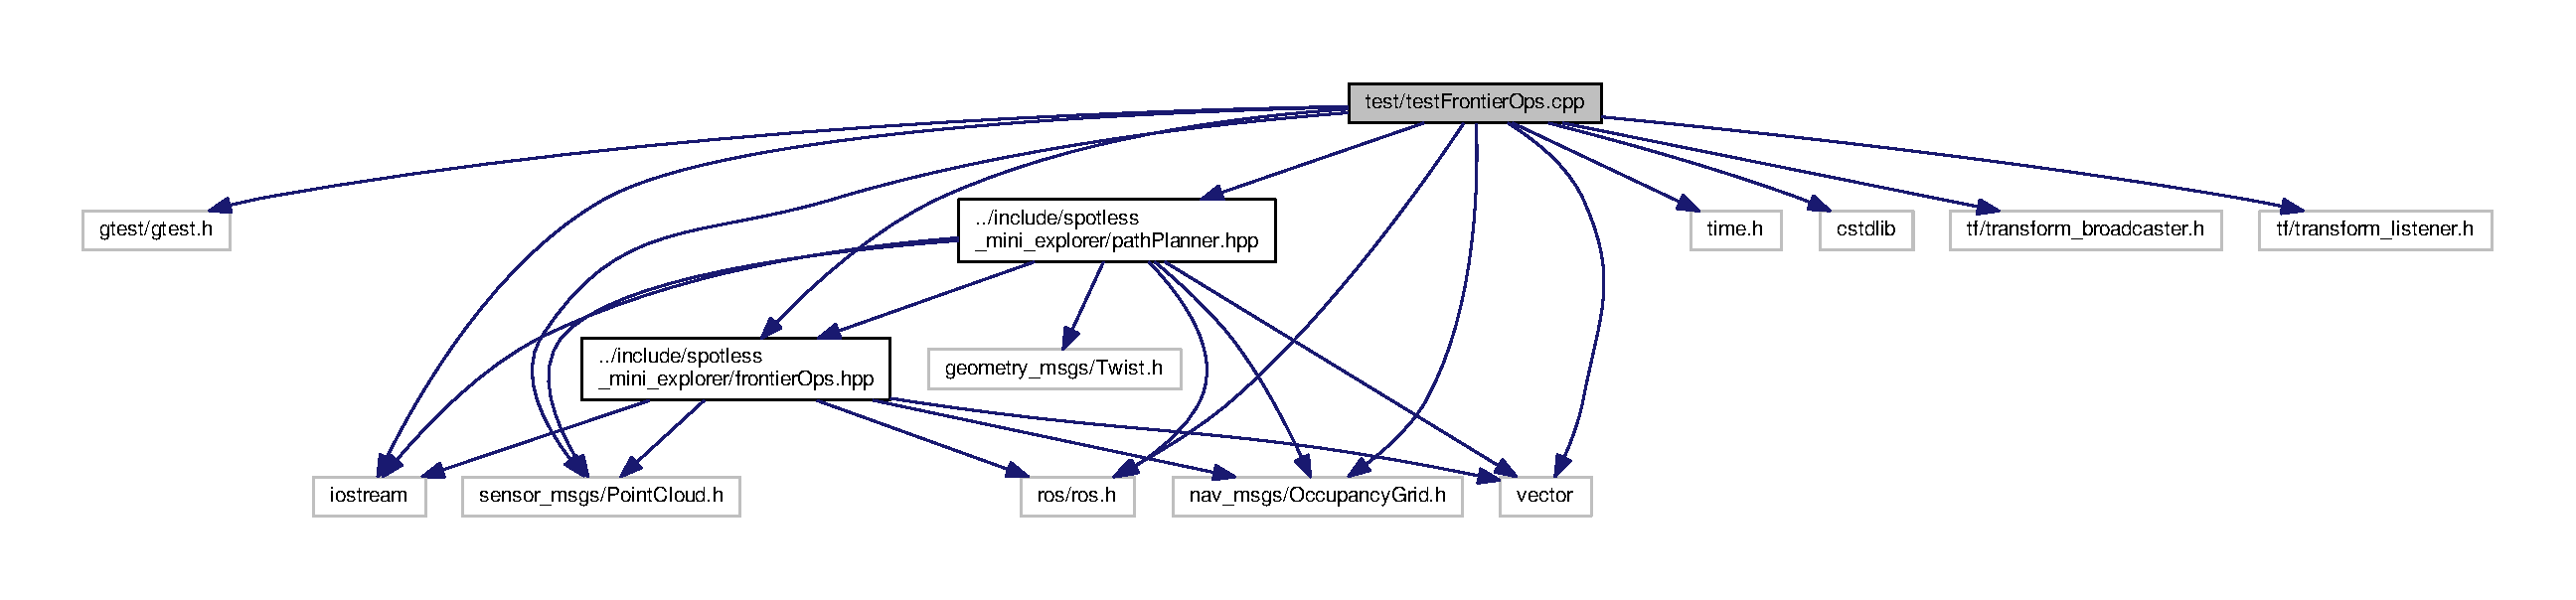
\includegraphics[width=350pt]{testFrontierOps_8cpp__incl}
\end{center}
\end{figure}
\subsection*{Functions}
\begin{DoxyCompactItemize}
\item 
\hyperlink{testFrontierOps_8cpp_a21163b06514292cecaecbe2532913b4d}{T\+E\+ST} (test\+Frontier, check\+Frontier\+Occupied\+More\+Than\+Thresh)\hypertarget{testFrontierOps_8cpp_a21163b06514292cecaecbe2532913b4d}{}\label{testFrontierOps_8cpp_a21163b06514292cecaecbe2532913b4d}

\begin{DoxyCompactList}\small\item\em Test for is\+Frontier() Checks if the given point is a frontier or not. Even if one frontier is present the test should be able to detect it and return appropriate state. \end{DoxyCompactList}\item 
\hyperlink{testFrontierOps_8cpp_a447d33cc7599a6d9dacf93ad9fce386d}{T\+E\+ST} (test\+Frontier, check\+Frontier\+No\+Data)\hypertarget{testFrontierOps_8cpp_a447d33cc7599a6d9dacf93ad9fce386d}{}\label{testFrontierOps_8cpp_a447d33cc7599a6d9dacf93ad9fce386d}

\begin{DoxyCompactList}\small\item\em Test for is\+Frontier() Checks if the given point is a frontier or not. Even no frontier is present the test should be able to detect it and return appropriate state. \end{DoxyCompactList}\item 
\hyperlink{testFrontierOps_8cpp_a6351645ca7214988cefa5ef24c5ce7aa}{T\+E\+ST} (test\+Process\+Frontier, get\+Frontiers)\hypertarget{testFrontierOps_8cpp_a6351645ca7214988cefa5ef24c5ce7aa}{}\label{testFrontierOps_8cpp_a6351645ca7214988cefa5ef24c5ce7aa}

\begin{DoxyCompactList}\small\item\em Test for process\+Frontiers() Test for processing frontiers. Checks for number of frontiers present in a map. \end{DoxyCompactList}\item 
\hyperlink{testFrontierOps_8cpp_a7410b9caa558583e4fdcc27243b09433}{T\+E\+ST} (test\+Distance, check\+Euclidean\+Distance)\hypertarget{testFrontierOps_8cpp_a7410b9caa558583e4fdcc27243b09433}{}\label{testFrontierOps_8cpp_a7410b9caa558583e4fdcc27243b09433}

\begin{DoxyCompactList}\small\item\em Test for get\+Distance() Checks the euclidean distance between two points. \end{DoxyCompactList}\end{DoxyCompactItemize}


\subsection{Detailed Description}
Frontier Ops is the base class and has important functions related to processing the frontiers. In this file we wish to test the functions of this class which can be isolated. Futher developments will be made. 

M\+IT License

Copyright (c) 2018 Sarthak Mahajan

Permission is hereby granted, free of charge, to any person obtaining a copy of this software and associated documentation files (the \char`\"{}\+Software\char`\"{}), to deal in the Software without restriction, including without limitation the rights to use, copy, modify, merge, publish, distribute, sublicense, and/or sell copies of the Software, and to permit persons to whom the Software is furnished to do so, subject to the following conditions\+:

The above copyright notice and this permission notice shall be included in all copies or substantial portions of the Software.

T\+HE S\+O\+F\+T\+W\+A\+RE IS P\+R\+O\+V\+I\+D\+ED \char`\"{}\+A\+S I\+S\char`\"{}, W\+I\+T\+H\+O\+UT W\+A\+R\+R\+A\+N\+TY OF A\+NY K\+I\+ND, E\+X\+P\+R\+E\+SS OR I\+M\+P\+L\+I\+ED, I\+N\+C\+L\+U\+D\+I\+NG B\+UT N\+OT L\+I\+M\+I\+T\+ED TO T\+HE W\+A\+R\+R\+A\+N\+T\+I\+ES OF M\+E\+R\+C\+H\+A\+N\+T\+A\+B\+I\+L\+I\+TY, F\+I\+T\+N\+E\+SS F\+OR A P\+A\+R\+T\+I\+C\+U\+L\+AR P\+U\+R\+P\+O\+SE A\+ND N\+O\+N\+I\+N\+F\+R\+I\+N\+G\+E\+M\+E\+NT. IN NO E\+V\+E\+NT S\+H\+A\+LL T\+HE A\+U\+T\+H\+O\+RS OR C\+O\+P\+Y\+R\+I\+G\+HT H\+O\+L\+D\+E\+RS BE L\+I\+A\+B\+LE F\+OR A\+NY C\+L\+A\+IM, D\+A\+M\+A\+G\+ES OR O\+T\+H\+ER L\+I\+A\+B\+I\+L\+I\+TY, W\+H\+E\+T\+H\+ER IN AN A\+C\+T\+I\+ON OF C\+O\+N\+T\+R\+A\+CT, T\+O\+RT OR O\+T\+H\+E\+R\+W\+I\+SE, A\+R\+I\+S\+I\+NG F\+R\+OM, O\+UT OF OR IN C\+O\+N\+N\+E\+C\+T\+I\+ON W\+I\+TH T\+HE S\+O\+F\+T\+W\+A\+RE OR T\+HE U\+SE OR O\+T\+H\+ER D\+E\+A\+L\+I\+N\+GS IN T\+HE S\+O\+F\+T\+W\+A\+RE. \begin{DoxyCopyright}{Copyright}
Copyright (c) 2018 Sarthak Mahajan
\end{DoxyCopyright}
\begin{DoxyAuthor}{Author}
Sarthak Mahajan 
\end{DoxyAuthor}

\hypertarget{testPathPlanner_8cpp}{}\section{test/test\+Path\+Planner.cpp File Reference}
\label{testPathPlanner_8cpp}\index{test/test\+Path\+Planner.\+cpp@{test/test\+Path\+Planner.\+cpp}}


Path Planner class is the derived class and primarily takes care of the call back function, for getting the map of the surrounding, and moving the robot.  


{\ttfamily \#include $<$gtest/gtest.\+h$>$}\\*
{\ttfamily \#include $<$ros/ros.\+h$>$}\\*
{\ttfamily \#include $<$vector$>$}\\*
{\ttfamily \#include \char`\"{}std\+\_\+srvs/\+Empty.\+h\char`\"{}}\\*
{\ttfamily \#include \char`\"{}../include/spotless\+\_\+mini\+\_\+explorer/path\+Planner.\+hpp\char`\"{}}\\*
Include dependency graph for test\+Path\+Planner.\+cpp\+:
\nopagebreak
\begin{figure}[H]
\begin{center}
\leavevmode
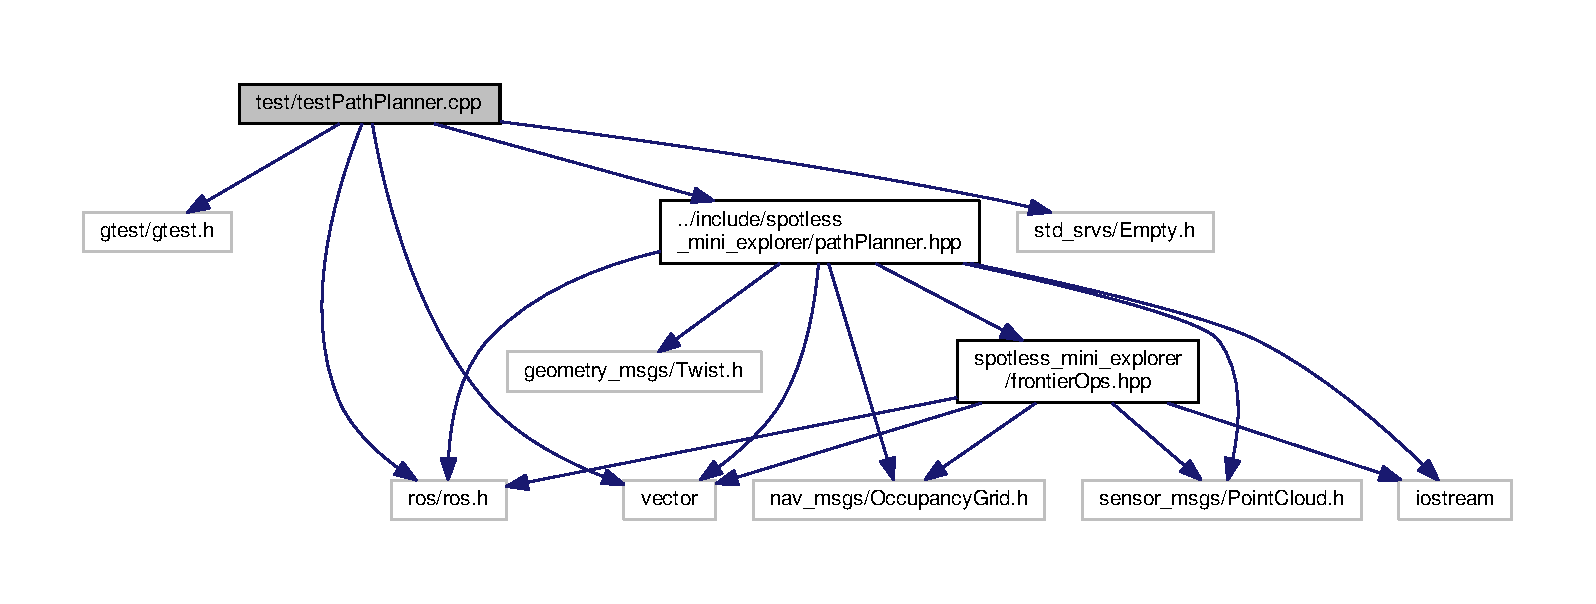
\includegraphics[width=350pt]{testPathPlanner_8cpp__incl}
\end{center}
\end{figure}
\subsection*{Functions}
\begin{DoxyCompactItemize}
\item 
\hyperlink{testPathPlanner_8cpp_a0f2d27d1923f83c738cff014110eddf2}{T\+E\+ST} (Test\+Path\+Planner\+Func, test\+Get\+Center\+Pt)\hypertarget{testPathPlanner_8cpp_a0f2d27d1923f83c738cff014110eddf2}{}\label{testPathPlanner_8cpp_a0f2d27d1923f83c738cff014110eddf2}

\begin{DoxyCompactList}\small\item\em Test for get\+Median() Checks if the center point of a frontier is as expected. \end{DoxyCompactList}\item 
\hyperlink{testPathPlanner_8cpp_a864a6402325d00f0c6cc05fbf9ee02fd}{T\+E\+ST} (Test\+Ros\+Activity, test\+Map\+CB)\hypertarget{testPathPlanner_8cpp_a864a6402325d00f0c6cc05fbf9ee02fd}{}\label{testPathPlanner_8cpp_a864a6402325d00f0c6cc05fbf9ee02fd}

\begin{DoxyCompactList}\small\item\em Test for full\+Scan() and update\+Map() Checks if the topic has been correctly set. Moreover it calls the call back function for map and also calls other connected functions. \end{DoxyCompactList}\end{DoxyCompactItemize}


\subsection{Detailed Description}
Path Planner class is the derived class and primarily takes care of the call back function, for getting the map of the surrounding, and moving the robot. 

M\+IT License

Copyright (c) 2018 Sarthak Mahajan

Permission is hereby granted, free of charge, to any person obtaining a copy of this software and associated documentation files (the \char`\"{}\+Software\char`\"{}), to deal in the Software without restriction, including without limitation the rights to use, copy, modify, merge, publish, distribute, sublicense, and/or sell copies of the Software, and to permit persons to whom the Software is furnished to do so, subject to the following conditions\+:

The above copyright notice and this permission notice shall be included in all copies or substantial portions of the Software.

T\+HE S\+O\+F\+T\+W\+A\+RE IS P\+R\+O\+V\+I\+D\+ED \char`\"{}\+A\+S I\+S\char`\"{}, W\+I\+T\+H\+O\+UT W\+A\+R\+R\+A\+N\+TY OF A\+NY K\+I\+ND, E\+X\+P\+R\+E\+SS OR I\+M\+P\+L\+I\+ED, I\+N\+C\+L\+U\+D\+I\+NG B\+UT N\+OT L\+I\+M\+I\+T\+ED TO T\+HE W\+A\+R\+R\+A\+N\+T\+I\+ES OF M\+E\+R\+C\+H\+A\+N\+T\+A\+B\+I\+L\+I\+TY, F\+I\+T\+N\+E\+SS F\+OR A P\+A\+R\+T\+I\+C\+U\+L\+AR P\+U\+R\+P\+O\+SE A\+ND N\+O\+N\+I\+N\+F\+R\+I\+N\+G\+E\+M\+E\+NT. IN NO E\+V\+E\+NT S\+H\+A\+LL T\+HE A\+U\+T\+H\+O\+RS OR C\+O\+P\+Y\+R\+I\+G\+HT H\+O\+L\+D\+E\+RS BE L\+I\+A\+B\+LE F\+OR A\+NY C\+L\+A\+IM, D\+A\+M\+A\+G\+ES OR O\+T\+H\+ER L\+I\+A\+B\+I\+L\+I\+TY, W\+H\+E\+T\+H\+ER IN AN A\+C\+T\+I\+ON OF C\+O\+N\+T\+R\+A\+CT, T\+O\+RT OR O\+T\+H\+E\+R\+W\+I\+SE, A\+R\+I\+S\+I\+NG F\+R\+OM, O\+UT OF OR IN C\+O\+N\+N\+E\+C\+T\+I\+ON W\+I\+TH T\+HE S\+O\+F\+T\+W\+A\+RE OR T\+HE U\+SE OR O\+T\+H\+ER D\+E\+A\+L\+I\+N\+GS IN T\+HE S\+O\+F\+T\+W\+A\+RE. \begin{DoxyCopyright}{Copyright}
Copyright (c) 2018 Sarthak Mahajan
\end{DoxyCopyright}
\begin{DoxyAuthor}{Author}
Sarthak Mahajan 
\end{DoxyAuthor}

%--- End generated contents ---

% Index
\backmatter
\newpage
\phantomsection
\clearemptydoublepage
\addcontentsline{toc}{chapter}{Index}
\printindex

\end{document}
